\let\negmedspace\undefined
\let\negthickspace\undefined
\documentclass[journal,12pt,onecolumn]{article}
\usepackage{cite}
\usepackage{amsmath,amssymb,amsfonts,amsthm}
\usepackage{algorithmic}
\usepackage{graphicx}
\usepackage{textcomp}
\usepackage{xcolor}
\usepackage{txfonts}
\usepackage{listings}
\usepackage{enumitem}
\usepackage{mathtools}
\usepackage{gensymb}
\usepackage{comment}
\usepackage[breaklinks=true]{hyperref}
\usepackage{tkz-euclide} 
\usepackage{listings}
\usepackage{gvv}                                        
%\def\inputGnumericTable{}                                 
\usepackage[latin1]{inputenc}     
\usepackage{xparse}
\usepackage{color}                                            
\usepackage{array}                                            
\usepackage{longtable}                                       
\usepackage{calc}                                             
\usepackage{multirow}
\usepackage{multicol}
\usepackage{hhline}                                           
\usepackage{ifthen}                                           
\usepackage{lscape}
\usepackage{tabularx}
\usepackage{array}
\usepackage{float}
\usepackage{bm}
\newtheorem{theorem}{Theorem}[section]
\newtheorem{problem}{Problem}
\newtheorem{proposition}{Proposition}[section]
\newtheorem{lemma}{Lemma}[section]
\newtheorem{corollary}[theorem]{Corollary}
\newtheorem{example}{Example}[section]
\newtheorem{definition}[problem]{Definition}
\newcommand{\BEQA}{\begin{eqnarray}}
\newcommand{\EEQA}{\end{eqnarray}}
\usepackage{float}
%\newcommand{\define}{\stackrel{\triangle}{=}}
\theoremstyle{remark}
\usepackage{ circuitikz }
%\newtheorem{rem}{Remark}
% Marks the beginning of the document
\begin{document}

\title{CE - 2025}
\author{EE25BTECH11043 - Nishid Khandagre}
\date{}
\maketitle

\renewcommand{\thefigure}{\theenumi}
\renewcommand{\thetable}{\theenumi}

\textbf{SESSION-1}


\begin{enumerate}

\item Is there any good show \underline{\hspace{2cm}} television tonight?
Select the most appropriate option to complete the above sentence.

\hfill{\brak{\text{GATE CE 2025}}}
\begin{enumerate}
\begin{multicols}{4}
    \item in
    \item at
    \item within
    \item on
    \end{multicols}
\end{enumerate}

\item As the police officer was found guilty of embezzlement, he was \underline{\hspace{2cm}} dismissed from the service in accordance with the Service Rules.
Select the most appropriate option to complete the above sentence.

\hfill{\brak{\text{GATE CE 2025}}}
\begin{enumerate}
\begin{multicols}{4}
    \item sumptuously
    \item brazenly
    \item unintentionally
    \item summarily
    \end{multicols}
\end{enumerate}

\item The sum of the following infinite series is:
\begin{align} \frac{1}{1!} + \frac{1}{2!} + \frac{1}{3!} + \frac{1}{4!} + \frac{1}{5!} + \dots \end{align}

\hfill{\brak{\text{GATE CE 2025}}}
\begin{enumerate}
\begin{multicols}{4}
    \item $\pi$
    \item $1+e$
    \item $e-1$
    \item $e$
    \end{multicols}
\end{enumerate}

\item A thin wire is used to construct all the edges of a cube of $1$ m side by bending, cutting and soldering the wire. If the wire is $12$ m long, what is the minimum number of cuts required to construct the wire frame to form the cube?

\hfill{\brak{\text{GATE CE 2025}}}
\begin{enumerate}
    \begin{multicols}{4}
    \item $3$
    \item $4$
    \item $6$
    \item $12$
    \end{multicols}
\end{enumerate}

\item The figures \figref{fig:q5} I, II and III are parts of a sequence. Which one of the following options comes next in the sequence at IV?
\begin{figure}[H]
    \centering
    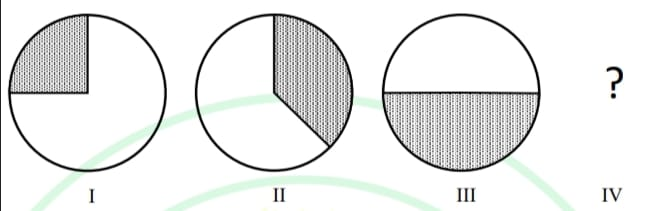
\includegraphics[width=0.7\columnwidth]{figs/q5-1.jpg}
    \caption{}
    \label{fig:q5}
\end{figure}

\hfill{\brak{\text{GATE CE 2025}}}
\begin{enumerate}
    \item \begin{figure}[H]
    \centering
    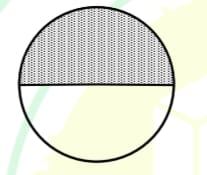
\includegraphics[width=0.4\columnwidth]{figs/1q-5a.jpg}
    \caption{}
    \label{fig:q5}
\end{figure}
\item \begin{figure}[H]
    \centering
    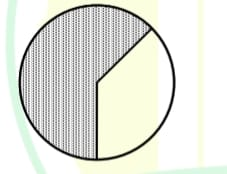
\includegraphics[width=0.4\columnwidth]{figs/1q-5b.jpg}
    \caption{}
    \label{fig:q5}
\end{figure}
\item \begin{figure}[H]
    \centering
    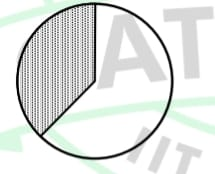
\includegraphics[width=0.4\columnwidth]{figs/1q-5c.jpg}
    \caption{}
    \label{fig:q5}
\end{figure}
\item \begin{figure}[H]
    \centering
    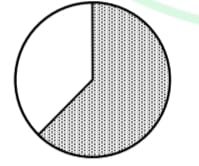
\includegraphics[width=0.4\columnwidth]{figs/1q-5d.jpg}
    \caption{}
    \label{fig:q5}
\end{figure}
\end{enumerate}

\item "Why do they pull down and do away with crooked streets, I wonder, which are my delight, and hurt no man living? Every day the wealthier nations are pulling down one or another in their capitals and their great towns: they do not know why they do it; neither do I. It ought to be enough, surely, to drive the great broad ways which commerce needs and which are the life-channels of a modern city, without destroying all history and all the humanity in between: the islands of the past." \brak{\text{From Hilaire Belloc's "The Crooked Streets"}}

Based only on the information provided in the above passage, which one of the following statements is true?

\hfill{\brak{\text{GATE CE 2025}}}
\begin{enumerate}
    \item The author of the passage takes delight in wondering.
    \item The wealthier nations are pulling down the crooked streets in their capitals.
    \item In the past, crooked streets were only built on islands.
    \item Great broad ways are needed to protect commerce and history.
\end{enumerate}

\item Rohit goes to a restaurant for lunch at about 1 PM. When he enters the restaurant, he notices that the hour and minute hands on the wall clock are exactly coinciding. After about an hour, when he leaves the restaurant, he notices that the clock hands are again exactly coinciding. How much time \brak{\text{in minutes}} did Rohit spend at the restaurant?

\hfill{\brak{\text{GATE CE 2025}}}
\begin{enumerate}
    \begin{multicols}{2}
    \item $64\frac{6}{11}$
    \item $66\frac{5}{13}$
    \item $65\frac{5}{11}$
    \item $66\frac{6}{13}$
    \end{multicols}
\end{enumerate}

\item A color model is shown in the figure \figref{fig:q8} with color codes: Yellow (Y), Magenta (M), Cyan (Cy), Red (R), Blue (Bl), Green (G), and Black (K). Which one of the following options displays the color codes that are consistent with the color model?
\begin{figure}[H]
    \centering
    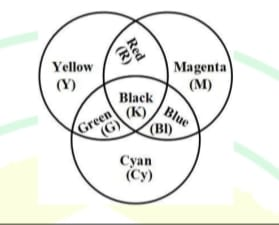
\includegraphics[width=0.4\columnwidth]{figs/1q-8.jpg}
    \caption{}
    \label{fig:q8}
\end{figure}

\hfill{\brak{\text{GATE CE 2025}}}
\begin{enumerate}
\begin{multicols}{2}
\item \begin{figure}[H]
    \centering
    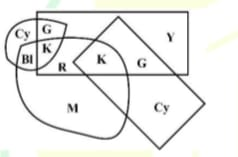
\includegraphics[width=0.5\columnwidth]{figs/1q-8a.jpg}
    \caption{}
    \label{fig:q8}
\end{figure}
\item \begin{figure}[H]
    \centering
    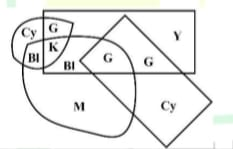
\includegraphics[width=0.5\columnwidth]{figs/1q-8b.jpg}
    \caption{}
    \label{fig:q8}
\end{figure}
\item \begin{figure}[H]
    \centering
    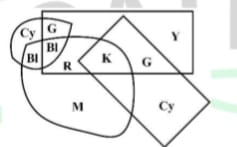
\includegraphics[width=0.5\columnwidth]{figs/1q-8c.jpg}
    \caption{}
    \label{fig:q8}
\end{figure}
\item \begin{figure}[H]
    \centering
    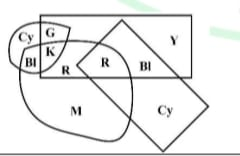
\includegraphics[width=0.5\columnwidth]{figs/1q-8d.jpg}
    \caption{}
    \label{fig:q8}
\end{figure}
\end{multicols}
\end{enumerate}

\item A circle with center at \brak{x,y} = \brak{0.5, 0} and radius = $0.5$ intersects with another circle with center at \brak{x, y} = \brak{1, 1} and radius = $1$ at two points. One of the points of intersection \brak{x, y} is:

\hfill{\brak{\text{GATE CE 2025}}}
\begin{enumerate}
    \begin{multicols}{2}
    \item \brak{0,0}
    \item \brak{0.2, 0.4}
    \item \brak{0.5, 0.5}
    \item \brak{1, 2}
    \end{multicols}
\end{enumerate}

\item An object is said to have an $n$-fold rotational symmetry if the object, rotated by an angle of $\frac{2\pi}{n}$, is identical to the original. Which one of the following objects exhibits 4-fold rotational symmetry about an axis perpendicular to the plane of the screen?
Note: The figures shown are representative.

\hfill{\brak{\text{GATE CE 2025}}}
\begin{enumerate}
\item \begin{figure}[H]
    \centering
    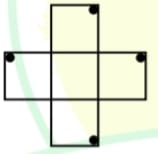
\includegraphics[width=0.5\columnwidth]{figs/1q-10a.jpg}
    \caption{}
    \label{fig:q8}
\end{figure}
\item \begin{figure}[H]
    \centering
    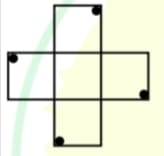
\includegraphics[width=0.5\columnwidth]{figs/1q-10b.jpg}
    \caption{}
    \label{fig:q8}
\end{figure}
\item \begin{figure}[H]
    \centering
    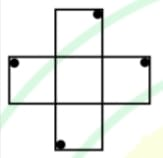
\includegraphics[width=0.5\columnwidth]{figs/1q-10c.jpg}
    \caption{}
    \label{fig:q8}
\end{figure}
\item \begin{figure}[H]
    \centering
    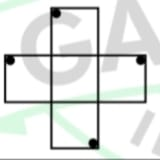
\includegraphics[width=0.5\columnwidth]{figs/1q-10d.jpg}
    \caption{}
    \label{fig:q8}
\end{figure}
\end{enumerate}

\item Suppose $\lambda$ is an eigenvalue of matrix $A$ and $x$ is the corresponding eigenvector. Let $x$ also be an eigenvector of the matrix $B = A - 2I$, where $I$ is the identity matrix. Then, the eigenvalue of $B$ corresponding to the eigenvector $x$ is equal to

\hfill{\brak{\text{GATE CE 2025}}}
\begin{enumerate}
    \begin{multicols}{2}
    \item $\lambda$
    \item $\lambda + 2$
    \item $2\lambda$
    \item $\lambda - 2$
    \end{multicols}
\end{enumerate}

\item Let $A = \myvec{1 & 1 \\ 1 & 3 \\ -2 & -3}$ and $b = \myvec{b_1 \\ b_2 \\ b_3}$. For $Ax=b$ to be solvable, which one of the following options is the correct condition on $b_1$, $b_2$, and $b_3$:

\hfill{\brak{\text{GATE CE 2025}}}
\begin{enumerate}
    \begin{multicols}{2}
    \item $b_1 + b_2 + b_3 = 1$
    \item $3b_1 + b_2 + 2b_3 = 0$
    \item $b_1 + 3b_2 + b_3 = 2$
    \item $b_1 + b_2 + b_3 = 2$
    \end{multicols}
\end{enumerate}

\item Which one of the following options is the correct Fourier series of the periodic function $f\brak{x}$ described below:
\begin{align} f\brak{x} = 
\begin{cases} 
0 & \text{if } -2 < x < -1 \\
2k & \text{if } -1 < x < 1 \\
0 & \text{if } 1 < x < 2 
\end{cases}
; \quad \text{period} = 4 \end{align}

\hfill{\brak{\text{GATE CE 2025}}}
\begin{enumerate}
    \item $f\brak{x} = \frac{k}{2} + \frac{2k}{\pi} \brak{\cos{\frac{\pi}{2}x} - \frac{1}{3}\cos{\frac{3\pi}{2}x} + \frac{1}{5}\cos{\frac{5\pi}{2}x} - \dots}$
    \item $f\brak{x} = \frac{k}{2} + \frac{2k}{\pi} \brak{\sin{\frac{\pi}{2}x} - \frac{1}{3}\sin{\frac{3\pi}{2}x} + \frac{1}{5}\sin{\frac{5\pi}{2}x} - \dots}$
    \item $f\brak{x} = k + \frac{4k}{\pi} \brak{\cos{\frac{\pi}{2}x} - \frac{1}{3}\cos{\frac{3\pi}{2}x} + \frac{1}{5}\cos{\frac{5\pi}{2}x} - \dots}$
    \item $f\brak{x} = k + \frac{4k}{\pi} \brak{\sin{\frac{\pi}{2}x} - \frac{1}{3}\sin{\frac{3\pi}{2}x} + \frac{1}{5}\sin{\frac{5\pi}{2}x} - \dots}$
\end{enumerate}

\item $X$ is a random variable that can take any one of the values $0, 1, 7, 11,$ and $12$. The probability mass function for $X$ is
$P\brak{X=0} = 0.4$; $P\brak{X=1} = 0.3$; $P\brak{X=7} = 0.1$;
$P\brak{X=11} = 0.1$; $P\brak{X=12} = 0.1$
Then, the variance of $X$ is

\hfill{\brak{\text{GATE CE 2025}}}
\begin{enumerate}
    \begin{multicols}{2}
    \item $20.81$
    \item $28.40$
    \item $31.70$
    \item $10.89$
    \end{multicols}
\end{enumerate}

\item As per IS 456:2000 provisions for two-way slabs with continuous edges, the longitudinal steel reinforcement to be provided in the edge strip is based on

\hfill{\brak{\text{GATE CE 2025}}}
\begin{enumerate}
    \item the calculated minimum bending moment
    \item the area of longitudinal steel provided in the middle strip in the shorter span
    \item the area of longitudinal steel provided in the middle strip in the longer span
    \item the prescribed minimum cross-sectional area of longitudinal steel for slabs
\end{enumerate}

\item Identify the FALSE statement from the following options:

\hfill{\brak{\text{GATE CE 2025}}}
\begin{enumerate}
    \item The compressive strength of a concrete test specimen can vary depending on its shape and size
    \item Air-dried and saturated test specimens show the same compressive strength for concrete
    \item Curing conditions, such as temperature and relative humidity, can influence the compressive strength of concrete
    \item Compressive strength depends on the water-to-binder ratio used in the concrete mixture
\end{enumerate}

\item The results of a consolidated drained triaxial test on a normally consolidated clay are shown in the figure \figref{fig:q17}. The angle of internal friction is
\begin{figure}[H]
    \centering
    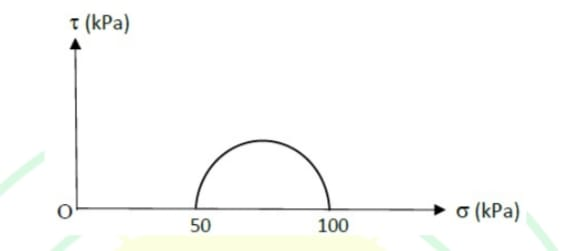
\includegraphics[width=0.7\columnwidth]{figs/1q-17.jpg}
    \caption{}
    \label{fig:q17}
\end{figure}

\hfill{\brak{\text{GATE CE 2025}}}
\begin{enumerate}
    \begin{multicols}{2}
    \item $\sin^{-1}\brak{\frac{1}{2}}$
    \item $\sin^{-1}\brak{\frac{1}{3}}$
    \item $\sin^{-1}\brak{\frac{2}{3}}$
    \item $\sin^{-1}\brak{\frac{3}{4}}$
    \end{multicols}
\end{enumerate}

\item The standard plasticity chart for the classification of a fine-grained soil is shown in the figure \figref{fig:q18}. As per the Indian standard soil classification system, X represents
\begin{figure}[H]
    \centering
    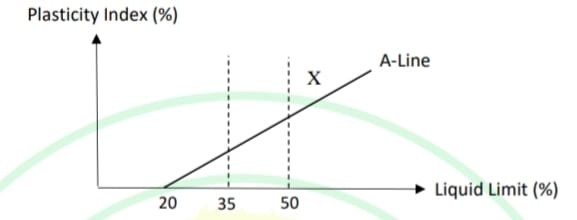
\includegraphics[width=0.7\columnwidth]{figs/1q-18.jpg}
    \caption{}
    \label{fig:q18}
\end{figure}

\hfill{\brak{\text{GATE CE 2025}}}
\begin{enumerate}
    \begin{multicols}{2}
    \item inorganic clay with medium plasticity
    \item inorganic silt with medium plasticity
    \item inorganic clay with high plasticity
    \item inorganic silt with high compressibility
    \end{multicols}
\end{enumerate}

\item For a flowing fluid, a dimensionless combination of velocity ($V$), length scale ($l$), and acceleration due to gravity ($g$) would be

\hfill{\brak{\text{GATE CE 2025}}}
\begin{enumerate}
    \begin{multicols}{2}
    \item $\frac{V^2}{gl}$
    \item $\frac{Vg}{l}$
    \item $\frac{gl^2}{V}$
    \item $\frac{l}{V^2g}$
    \end{multicols}
\end{enumerate}

\item To derive the total flood hydrograph at a catchment outlet from an isolated storm, the order in which the following methods are applied, from the first method to the last method, is
P. Obtaining the hyetograph
Q. Addition of baseflow
R. Estimation of initial and infiltration losses
S. Application of unit hydrograph

\hfill{\brak{\text{GATE CE 2025}}}
\begin{enumerate}
    \begin{multicols}{2}
    \item PRSQ
    \item PQRS
    \item RPSQ
    \item PSQR
    \end{multicols}
\end{enumerate}

\item Fecal Coliform (FC) concentration in river water was measured as 10780 cfu/100 ml. The FC concentration after the conventional water treatment, but before chlorination, was measured as 23 cfu/100 ml. The 'Log Kill' (inactivation) of FC due to the conventional water treatment is closest to

\hfill{\brak{\text{GATE CE 2025}}}
\begin{enumerate}
    \begin{multicols}{2}
    \item 4.00
    \item 2.50
    \item 2.67
    \item 3.00
    \end{multicols}
\end{enumerate}

\item A hydrocarbon ($C_n H_m$) is burnt in air ($O_2 + 3.78 N_2$). The stoichiometric fuel to air mass ratio for this process is
Note: Atomic Weight: C(12), H(1)
Effective Molecular Weight: Air(28.8)
Ignore any conversion of $N_2$ in air to the oxides of nitrogen ($NO_x$)

\hfill{\brak{\text{GATE CE 2025}}}
\begin{enumerate}
    \begin{multicols}{2}
    \item $0.0291 \frac{\brak{4n+m}}{\brak{12n+m}}$
    \item $34.42 \frac{\brak{12n+m}}{\brak{4n+m}}$
    \item $34.42 \frac{\brak{4n+m}}{\brak{12n+m}}$
    \item $0.0291 \frac{\brak{12n+m}}{\brak{4n+m}}$
    \end{multicols}
\end{enumerate}

\item All the vehicles that come during a particular peak hour come during a 10-minute period within this hour. The 15-minute peak hour factor for this peak hour is

\hfill{\brak{\text{GATE CE 2025}}}
\begin{enumerate}
    \begin{multicols}{2}
    \item 0.25
    \item 0.167
    \item 0.75
    \item 1.0
    \end{multicols}
\end{enumerate}

\item In the context of testing bitumen, which one of the following statements is FALSE:

\hfill{\brak{\text{GATE CE 2025}}}
\begin{enumerate}
    \item The depth of penetration of needle in the standard penetration test is measured in the units of one-tenth of millimeter
    \item Softening point is measured using a ring and ball apparatus
    \item Softening point is measured in the units of time
    \item Ductility is measured in the units of length
\end{enumerate}

\item The maximum degree of the curve that can be used for railways in a mountainous region is

\hfill{\brak{\text{GATE CE 2025}}}
\begin{enumerate}
    \begin{multicols}{2}
    \item 10
    \item 20
    \item 50
    \item 40
    \end{multicols}
\end{enumerate}

\item If the horizontal distance between a staff point and the point of observation is $d$, the error due to the curvature of earth is proportional to

\hfill{\brak{\text{GATE CE 2025}}}
\begin{enumerate}
    \begin{multicols}{2}
    \item $d$
    \item $\frac{1}{d}$
    \item $d^2$
    \item $\frac{1}{d^2}$
    \end{multicols}
\end{enumerate}

\item If the quadrantal bearing of a line is N30$\degree$W, then the whole circle bearing of the line is

\hfill{\brak{\text{GATE CE 2025}}}
\begin{enumerate}
    \begin{multicols}{2}
    \item 120$\degree$
    \item 210$\degree$
    \item 300$\degree$
    \item 330$\degree$
    \end{multicols}
\end{enumerate}

\item Which of the following equations belong/belongs to the class of second-order, linear, homogeneous partial differential equations:

\hfill{\brak{\text{GATE CE 2025}}}
\begin{enumerate}
    \item $\frac{\partial^2 u}{\partial t^2} = c^2 \brak{\frac{\partial^2 u}{\partial x^2} + \frac{\partial^2 u}{\partial y^2}} + xy$
    \item $\frac{\partial^2 u}{\partial x^2} + \frac{\partial^2 u}{\partial y^2} + \frac{\partial^2 u}{\partial z^2} = 0$
    \item $\frac{\partial u}{\partial t} = c \frac{\partial u}{\partial x}$
    \item $\brak{\frac{\partial^2 u}{\partial t^2}}^2 = c^2 \frac{\partial^2 u}{\partial x^2}$
\end{enumerate}

\item Consider the frame shown in the figure \figref{fig:q29} under the loading of 100 kN.m couples at the joints B and G. Considering only the effects of flexural deformations, which of the following statements is/are true:
\begin{figure}[H]
    \centering
    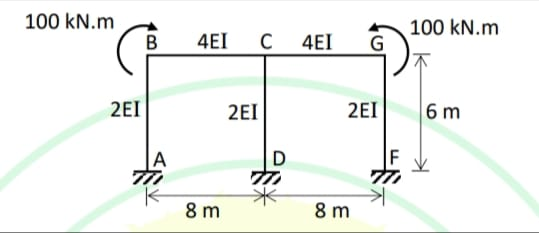
\includegraphics[width=0.7\columnwidth]{figs/1q-29.jpg}
    \caption{}
    \label{fig:q29}
\end{figure}

\hfill{\brak{\text{GATE CE 2025}}}
\begin{enumerate}
    \item Axial force is zero in the member CD
    \item Shear force is zero in the member CD
    \item There is no rotation in the joint C
    \item The magnitude of bending moment developed in the member BC at the end C is more than 50 kN.m
\end{enumerate}

\item For the Bernoulli's equation to be applicable in a fluid flow situation, which of the following conditions is/are to be satisfied:

\hfill{\brak{\text{GATE CE 2025}}}
\begin{enumerate}
    \item Fluid should be frictionless
    \item Fluid should be incompressible
    \item Flow should be steady
    \item Flow should be rotational
\end{enumerate}

\item The Surface Overflow Rate (SOR) in a rectangular sedimentation tank is 45 m$^3$/m$^2$/d. Minimum diameters of spherical inorganic and organic particles expected to be completely removed in this tank are calculated. Assume that Stoke's law is applicable. Which of the following options is/are correct:
Specific gravity of inorganic particles = 2.65
Specific gravity of organic particles = 1.20
Acceleration due to gravity (g) = 9.81 m/s$^2$
Kinematic viscosity ($\nu$) = $1 \times 10^{-6}$ m$^2$/s

\hfill{\brak{\text{GATE CE 2025}}}
\begin{enumerate}

    \item Minimum diameter of inorganic particles is 24 $\mu$m
    \item Minimum diameter of organic particles is 69 $\mu$m
    \item Minimum diameter of inorganic particles is 15 $\mu$m
    \item Minimum diameter of organic particles is 55 $\mu$m
   
\end{enumerate}

\item Aeration is employed as a treatment option for the removal of several pollutants from contaminated water.
Identify the pollutant(s), where aeration is employed as a part of their removal:

\hfill{\brak{\text{GATE CE 2025}}}
\begin{enumerate}
    \begin{multicols}{2}
    \item Iron
    \item Cadmium
    \item Manganese
    \item Zinc
    \end{multicols}
\end{enumerate}

\item If the weights retained on the 2.36 mm, 1.18 mm, 600 $\mu$m, and 300 $\mu$m sieves are 30\%, 35\%, 15\%, and 20\%, respectively, of the total weight of an aggregate sample, then the fineness modulus of the sample is \underline{\hspace{2cm}} \brak{\text{rounded off to 2 decimal places}}.

\hfill{\brak{\text{GATE CE 2025}}}

\item A water resources project with an expected life of 25 years has to be designed for an acceptable risk of 5\% against a design flood. The return period for the design flood (in years) is \underline{\hspace{2cm}} \brak{\text{rounded off to the nearest integer}}.

\hfill{\brak{\text{GATE CE 2025}}}

\item Road A and Road B are joined by a circular horizontal curve of radius 200 m as shown in the figure \figref{fig:q35}. Road A and Road B are tangential to the curve at the points C and D, respectively. Had the curve not been there, straight roads A and B would have met at the point E. The distance from C to E is 92 m. The value of angle $\theta$ \brak{\text{in degrees}} is \underline{\hspace{2cm}} \brak{\text{rounded off to 1 decimal place}}.
Note: The value of angle $\theta$ is to be calculated only from the consideration of Euclidean geometry and the data given in the problem.
\begin{figure}[H]
    \centering
    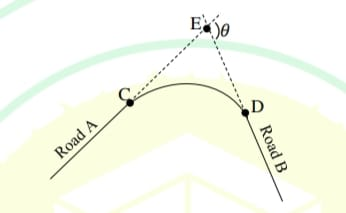
\includegraphics[width=0.7\columnwidth]{figs/1q-35.jpg}
    \caption{}
    \label{fig:q35}
\end{figure}

\hfill{\brak{\text{GATE CE 2025}}}

\item The value of $\lim_{x \to \infty} \brak{x - \sqrt{x^2+x}}$ is equal to

\hfill{\brak{\text{GATE CE 2025}}}
\begin{enumerate}
    \begin{multicols}{2}
    \item -1
    \item -0.5
    \item -2
    \item 0
    \end{multicols}
\end{enumerate}

\item In the rigid-jointed frame shown in the figure \figref{fig:q37}, the distribution factor of the member AD is closest to
\begin{figure}[H]
    \centering
    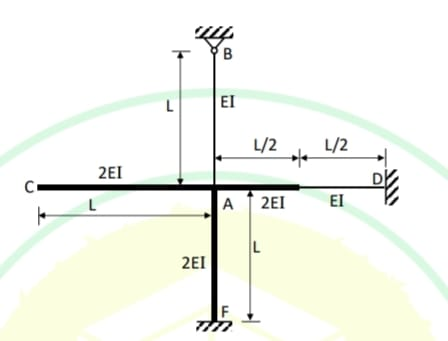
\includegraphics[width=0.7\columnwidth]{figs/1q-37.jpg}
    \caption{}
    \label{fig:q37}
\end{figure}

\hfill{\brak{\text{GATE CE 2025}}}
\begin{enumerate}
    \begin{multicols}{2}
    \item 0.254
    \item 0.267
    \item 0.398
    \item 0.421
    \end{multicols}
\end{enumerate}

\item In an oedometer apparatus a specimen of fully saturated clay has been consolidated under a vertical pressure of 100 kPa and is at equilibrium state. Immediately on increasing the vertical pressure to 150 kPa, the effective stress $\sigma'$ and excess pore water pressure $\Delta u$ will be

\hfill{\brak{\text{GATE CE 2025}}}
\begin{enumerate}
    \item $\sigma' = 50 \text{ kPa}, \Delta u = 100 \text{ kPa}$
    \item $\sigma' = 100 \text{ kPa}, \Delta u = 50 \text{ kPa}$
    \item $\sigma' = 150 \text{ kPa}, \Delta u = 50 \text{ kPa}$
    \item $\sigma' = 100 \text{ kPa}, \Delta u = 150 \text{ kPa}$
\end{enumerate}

\item The mean rainfall over a catchment has to be estimated. The data for four rain gauges located in and around the catchment is listed in the table. Which one of the following statements is correct:
\begin{table}[H]
    \centering
    \begin{tabular}{|l|c|c|c|c|}
        \hline
        \textbf{Rain gauge station} & P & Q & R & S \\
        \hline
        \textbf{Whether located inside the} & Yes & Yes & Yes & No \\
        \textbf{catchment} & & & & \\
        \hline
        \textbf{Thiessen weightage factor} & 0.25 & 0.50 & 0.10 & 0.15 \\
        \hline
        \textbf{Rainfall (mm)} & 100 & 110 & 100 & 125 \\
        \hline
    \end{tabular}
    \caption{}
    \label{tab:q39}
\end{table}

\hfill{\brak{\text{GATE CE 2025}}}
\begin{enumerate}
    \item The estimate obtained from the Thiessen-mean method is greater than that obtained using the arithmetic-mean method
    \item The estimate obtained from the Thiessen-mean method is equal to that obtained using the arithmetic-mean method
    \item The estimate obtained from the Thiessen-mean method is less than that obtained using the arithmetic-mean method
    \item The Thiessen-mean method cannot be applied in this case
\end{enumerate}

\item The speed-density relation on a one-way, single lane road is shown in the figure \figref{fig:q40}, where speed $u$ is in km/hour and density $k$ is in vehicles/km. The maximum flow (in vehicles/hour) on this road is
\begin{figure}[H]
    \centering
    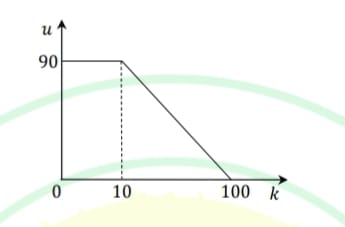
\includegraphics[width=0.7\columnwidth]{figs/1q-40.jpg}
    \caption{}
    \label{fig:q40}
\end{figure}

\hfill{\brak{\text{GATE CE 2025}}}
\begin{enumerate}
    \begin{multicols}{2}
    \item 2500
    \item 900
    \item 2250
    \item 2000
    \end{multicols}
\end{enumerate}

\item Consider the beam ACDEB given in the figure \figref{fig:q41}. Which of the following statements is/are correct:
\begin{figure}[H]
    \centering
    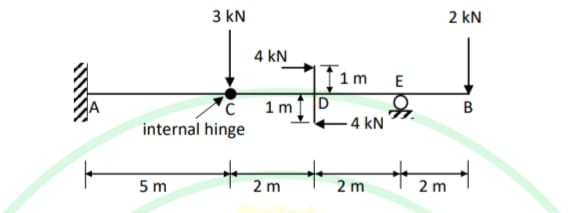
\includegraphics[width=0.7\columnwidth]{figs/1q-41.jpg}
    \caption{}
    \label{fig:q41}
\end{figure}

\hfill{\brak{\text{GATE CE 2025}}}
\begin{enumerate}
    \item Bending moment is zero between the points A and C
    \item There is a sudden jump in shear force at the point D
    \item There is a sudden jump in bending moment at the point E
    \item Bending moment is zero somewhere between the points D and E
\end{enumerate}

\item In the context of construction project management, which of the following statements is/are true:

\hfill{\brak{\text{GATE CE 2025}}}
\begin{enumerate}
    \item A dummy activity will consume time and resources
    \item The programme evaluation and review technique (PERT) is best suited for projects with large uncertainties in the duration of activities
    \item A Gantt chart is commonly used for identifying the 'critical path' of activities in a project
    \item Free float is the amount of time by which the start of an activity can be delayed without causing a delay in the start of a following activity
\end{enumerate}

\item Lacey's regime equations, followed in India for making scour calculations while designing hydraulic structures across alluvial channels, are given below. Regarding these equations, which of the following statements is/are true:
\begin{align*}
    D &= 0.470 \times \brak{\frac{Q}{f_s}}^{1/3} \\
    P &= 4.75 \times \sqrt{Q} \\
    f_s &= 1.76 \times \sqrt{d}
\end{align*}
where, $Q$ is discharge and $f_s$ is silt factor.

\hfill{\brak{\text{GATE CE 2025}}}
\begin{enumerate}
    \item $D$ is the depth of scour below the existing riverbed
    \item $P$ is the Lacey's waterway width
    \item $d$ is the average grain size diameter of the bed material in centimetres
    \item $D$ is the depth of scour below the design flood level
\end{enumerate}

\item MgCl$_2$ and CaSO$_4$ salts are added to 1 litre of distilled deionized water and mixed until completely dissolved. Total Dissolved Solids (TDS) concentration is 500 mg/l, and Total Hardness (TH) is 400 mg/l (as CaCO$_3$). The amounts of MgCl$_2$ and CaSO$_4$ added are calculated (rounded off to the nearest integer). Which of the following options is/are true:
Atomic weights: Ca(40), Mg(24), S(32), O(16), Cl(35.5), C(12)

\hfill{\brak{\text{GATE CE 2025}}}
\begin{enumerate}
    \begin{multicols}{2}
    \item Amount of MgCl$_2$ added is 143 mg
    \item Amount of CaSO$_4$ added is 357 mg
    \item Amount of MgCl$_2$ added is 103 mg
    \item Amount of CaSO$_4$ added is 397 mg
    \end{multicols}
\end{enumerate}

\item A facultative pond system is employed for wastewater treatment. Which of the following statements is/are true:

\hfill{\brak{\text{GATE CE 2025}}}
\begin{enumerate}
    \item The dissolved oxygen concentration will be high during daytime compared to night-time
    \item The pH will be high during daytime compared to night-time
    \item The dissolved oxygen concentration will be low during daytime compared to night-time
    \item The pH will be low during daytime compared to night-time
\end{enumerate}

\item Organic fraction of municipal solid waste (OFMSW) with bulk density of 315 kg/m$^3$ and water content of 30\% is mixed with municipal sludge of bulk density 700 kg/m$^3$ and water content of 70\%, such that the water content of the mixture is 40\%. The amount (in kg) of sludge to be mixed per kg of OFMSW (rounded off to 2 decimal places) and the density of the mixture (in kg/m$^3$) (rounded off to the nearest integer) are calculated. Which of the following options is/are true:

\hfill{\brak{\text{GATE CE 2025}}}
\begin{enumerate}
  
    \item 0.33 kg of sludge added per kg of OFMSW
    \item Density of the mixture is 365 kg/m$^3$
    \item 0.66 kg of sludge added per kg of OFMSW
    \item Density of the mixture is 450 kg/m$^3$
  
\end{enumerate}

\item Let $y$ be the solution of the initial value problem $y'' + 0.8y' + 0.16y = 0$, where $y\brak{0} = 3$ and $y'\brak{0} = 4.5$. Then, $y\brak{1}$ is equal to \underline{\hspace{2cm}} \brak{\text{rounded off to 1 decimal place}}.

\hfill{\brak{\text{GATE CE 2025}}}

\item The maximum value of the function $h\brak{x} = -x^3 + 2x^2$ in the interval [-1,1.5] is equal to \underline{\hspace{2cm}} \brak{\text{rounded off to 1 decimal place}}.

\hfill{\brak{\text{GATE CE 2025}}}

\item Consider the differential equation given below. Using the Euler method with the step size \brak{h} of 0.5, the value of $y$ at $x=1.0$ is equal to \underline{\hspace{2cm}} \brak{\text{rounded off to 1 decimal place}}.
\begin{align} \frac{dy}{dx} = y + 2x - x^2; \quad y\brak{0} = 1 \quad \brak{0 \le x < \infty} \end{align}

\hfill{\brak{\text{GATE CE 2025}}}

\item For the beam and loading shown in the figure \figref{fig:q50} , the second derivative of the deflection curve of the beam at the mid-point of AC is given by $\alpha M_o / 8EI$. The value of $\alpha$ is \underline{\hspace{2cm}} \brak{\text{rounded off to the nearest integer}}.
\begin{figure}[H]
    \centering
    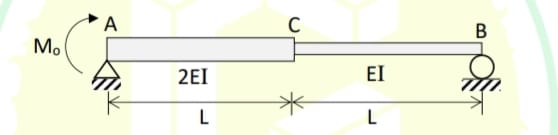
\includegraphics[width=0.7\columnwidth]{figs/1q-50.jpg}
    \caption{}
    \label{fig:q50}
\end{figure}

\hfill{\brak{\text{GATE CE 2025}}}

\item Consider the rigid bar ABC supported by the pin-jointed links BD and CE and subjected to a load P at the end A, as shown in the figure \figref{fig:q51}. The axial rigidities of BD and CE are 22500 kN and 15000 kN, respectively. If CE elongates by 5 mm due to the load P, the magnitude of the downward deflection (in mm) of the end A would be \underline{\hspace{2cm}} \brak{\text{rounded off to the nearest integer}}.
\begin{figure}[H]
    \centering
    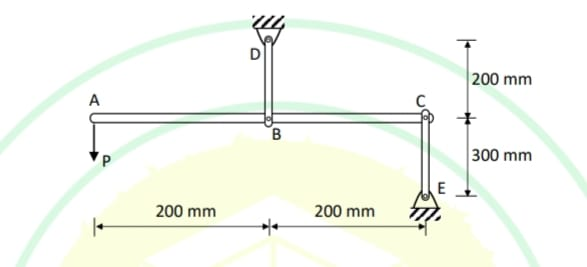
\includegraphics[width=0.7\columnwidth]{figs/1q-51.jpg}
    \caption{}
    \label{fig:q51}
\end{figure}

\hfill{\brak{\text{GATE CE 2025}}}

\item Consider a reinforced concrete beam section of 300 mm width and 700 mm depth. The beam is reinforced with the tension steel of 2000 mm$^2$ area at an effective cover of 50 mm. Concrete in the tension zone is assumed to be cracked. Assume the modular ratio of 12 and Young's modulus of 200 GPa for steel. When the extreme fibre in the compression zone undergoes the strain of 0.0004 due to the applied bending moment, the stress in the steel (in MPa) is \underline{\hspace{2cm}} \brak{\text{rounded off to the nearest integer}}.

\hfill{\brak{\text{GATE CE 2025}}}

\item Consider the beam section shown in the figure \figref{fig:q53}, with $\bar{y}$ indicating the depth of neutral axis (NA). The section is only subjected to an increasing bending moment. It is given that $\bar{y} = 18.75$ mm, when the section has not yielded at the top and bottom fibres. Further, $\bar{y}$ decreases to 5 mm, when the entire section has yielded. The shape factor of the section is \underline{\hspace{2cm}} \brak{\text{rounded off to 2 decimal places}}.
\begin{figure}[H]
    \centering
    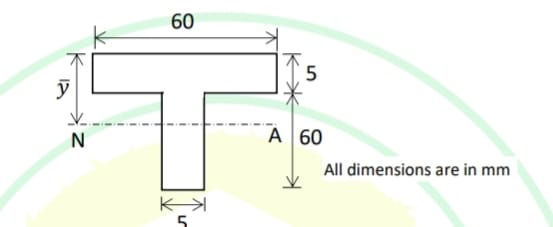
\includegraphics[width=0.7\columnwidth]{figs/1q-53.jpg}
    \caption{}
    \label{fig:q53}
\end{figure}

\hfill{\brak{\text{GATE CE 2025}}}

\item Consider the built-up column made of two I-sections as shown in the figure \figref{fig:q54}, with each batten plate bolted to a component I-section of the column through 6 black bolts. Each connection of the batten plate with the component section is to be designed for a longitudinal shear of 70 kN and moment of 10 kN.m. The minimum bolt value required (in kN) is \underline{\hspace{2cm}} \brak{\text{rounded off to the nearest integer}}.
\begin{figure}[H]
    \centering
    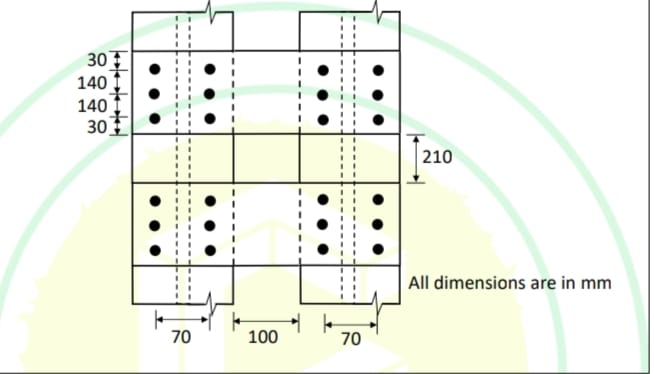
\includegraphics[width=0.7\columnwidth]{figs/1q-54.jpg}
    \caption{}
    \label{fig:q54}
\end{figure}

\hfill{\brak{\text{GATE CE 2025}}}

\item A cut slope is made in a silty clay soil for a new road project, as shown in the figure \figref{fig:q55}. The locations of ground water table (GWT) and potential failure surface are shown in the figure. After the cut is made, the excess pore water pressure is fully dissipated, and the shear stress at the point A is 60 kN/m$^2$. The factor of safety at the point A for long-term stability is \underline{\hspace{2cm}} \brak{\text{rounded off to 2 decimal places}}.
Note:
Shear strength properties of silty clay: $c' = 15$ kN/m$^2$, $\phi' = 15\degree$, and $c_u = 75$ kN/m$^2$
Unit weight of soil above the GWT ($\gamma$) = 19 kN/m$^3$
Unit weight of soil below the GWT ($\gamma_{sat}$) = 20 kN/m$^3$
Unit weight of water ($\gamma_w$) = 9.81 kN/m$^3$
\begin{figure}[H]
    \centering
    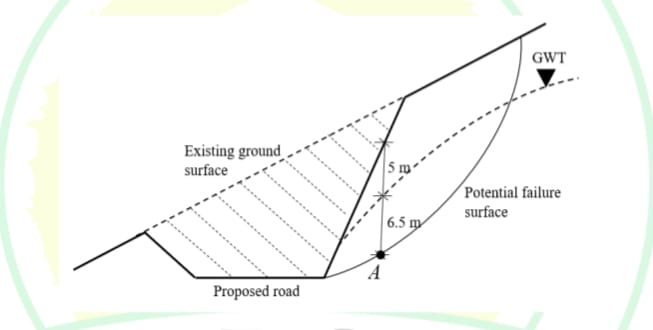
\includegraphics[width=0.7\columnwidth]{figs/1q-55.jpg}
    \caption{}
    \label{fig:q55}
\end{figure}

\hfill{\brak{\text{GATE CE 2025}}}

\item A 6 m $\times$ 6 m square footing constructed in clay is subjected to a vertical load of 2500 kN at its centre. The base of the footing is 2 m below the ground surface, as shown in the figure \figref{fig:q56}. The footing is made of 2 m thick concrete. The ground water table is at a great depth. Considering Terzaghi's bearing capacity theory, the factor of safety of footing against the bearing capacity failure is \underline{\hspace{2cm}} \brak{\text{rounded off to 2 decimal places}}.
Note:
Unit weight of concrete = 24 kN/m$^3$
Properties of clay: $c = 50$ kN/m$^2$, $\phi = 0\degree$, and $\gamma = 19$ kN/m$^3$
For $\phi = 0\degree$: $N_c = 5.7$, $N_q = 1$, $N_\gamma = 0$
\begin{figure}[H]
    \centering
    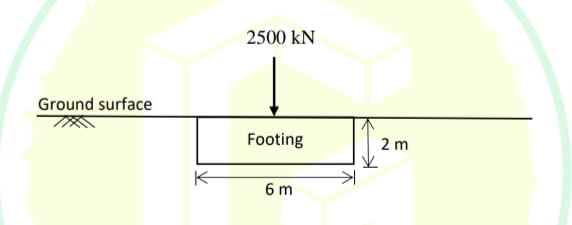
\includegraphics[width=0.7\columnwidth]{figs/1q-56.jpg}
    \caption{}
    \label{fig:q56}
\end{figure}

\hfill{\brak{\text{GATE CE 2025}}}

\item A clayey soil has a moisture content of 18\%, a specific gravity of soil solids of 2.74, and a degree of saturation of 65\%. The soil soaks up water during a rain event, and the degree of saturation increases to 85.2\%. The change of the volume during the soaking is negligible. The new moisture content (in \%) of the soil will be \underline{\hspace{2cm}} \brak{\text{rounded off to 2 decimal places}}.

\hfill{\brak{\text{GATE CE 2025}}}

\item A single pile with 450 mm diameter has been driven into a homogeneous clay layer, which has an undrained cohesion ($c_u$) of 20 kPa and unit weight of 18 kN/m$^3$. The ground water table is found to be at the surface of the clay layer. The adhesion factor ($\alpha$) of the soil is 0.95 and bearing capacity factor ($N_c$) is 9. The pile is supporting a column load of 144 kN with a factor of safety of 3.0 against ultimate axial pile capacity in compression.
The required embedment depth of the pile (in m) is \underline{\hspace{2cm}} \brak{\text{rounded off to the nearest integer}}.

\hfill{\brak{\text{GATE CE 2025}}}

\item Two soils of permeabilities $k_1$ and $k_2$ are placed in a horizontal flow apparatus, as shown in the figure \figref{fig:q59}. For Soil 1, $L_1 = 50$ cm, and $k_1 = 0.055$ cm/s; for Soil 2, $L_2 = 30$ cm, and $k_2 = 0.035$ cm/s. The cross sectional area of the horizontal pipe is 100 cm$^2$, and the head difference ($\Delta h$) is 150 cm. The discharge (in cm$^3$/s) through the soils is \underline{\hspace{2cm}} \brak{\text{rounded off to 2 decimal places}}.
\begin{figure}[H]
    \centering
    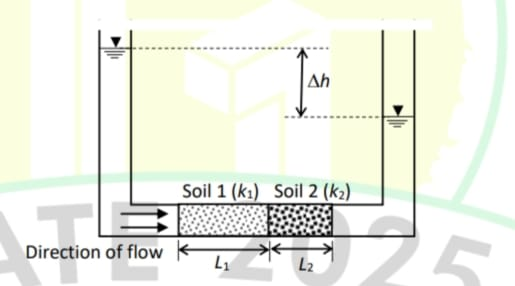
\includegraphics[width=0.7\columnwidth]{figs/1q-59.jpg}
    \caption{}
    \label{fig:q59}
\end{figure}

\hfill{\brak{\text{GATE CE 2025}}}

\item A hydraulic jump is formed in a 5 m wide rectangular channel, which has a horizontal bed and is carrying a discharge of 15 m$^3$/s. The depth of water upstream of the jump is 0.5 m. The power dissipated by the jump (in kW) is \underline{\hspace{2cm}} \brak{\text{rounded off to the nearest integer}}.
Note:
Acceleration due to gravity = 9.81 m/s$^2$
Density of water = 1000 kg/m$^3$
Kinetic energy correction factor = 1.0

\hfill{\brak{\text{GATE CE 2025}}}

\item A symmetrical trapezoidal canal is 100 km long. The bottom width is 10 m and the side slope is 1 Horizontal : 1 Vertical. The average flow depth in the canal is 2.5 m throughout the month of April. The measurement from a Class-A evaporimeter in the vicinity of the canal indicated an average evaporation rate of 0.5 cm/day in April.
The volume of water evaporated from the canal (in m$^3$) in the month of April is close to \underline{\hspace{2cm}} $\times 10^3$ \brak{\text{rounded off to 1 decimal place}}.

\hfill{\brak{\text{GATE CE 2025}}}

\item A 5.0 m wide rectangular channel carries a discharge of 10 m$^3$/s at a depth of 1.5 m under uniform flow. To produce critical flow conditions without affecting the upstream conditions, the channel bottom elevation should be raised (in m) by \underline{\hspace{2cm}} \brak{\text{rounded off to 2 decimal places}}.
Assume that there is no loss of head at the raise, kinetic energy correction factor is 1.0, and acceleration due to gravity is 9.81 m/s$^2$.

\hfill{\brak{\text{GATE CE 2025}}}

\item A one-way, single lane road has traffic that consists of 30\% trucks and 70\% cars. The speed of trucks (in km/h) is a uniform random variable on the interval (30, 60), and the speed of cars (in km/h) is a uniform random variable on the interval (40, 80). The speed limit on the road is 50 km/h. The percentage of vehicles that exceed the speed limit is \underline{\hspace{2cm}} \brak{\text{rounded off to 1 decimal place}}.
Note: $X$ is a uniform random variable on the interval ($\alpha, \beta$), if its probability density function is given by
\begin{align} 
f(x) = 
\begin{cases} 
\frac{1}{\beta - \alpha} & a < x < \beta \\
0 & \text{otherwise}
\end{cases}
\end{align}

\hfill{\brak{\text{GATE CE 2025}}}

\item In levelling between two points A and B on the opposite banks of a river, the readings are taken by setting the instrument both at A and B, as shown in the table. If the RL of A is 150.000 m, the RL of B (in m) is \underline{\hspace{2cm}} \brak{\text{rounded off to 3 decimal places}}.
\begin{table}[H]
    \centering
    \begin{tabular}{|c|c|c|}
        \hline
        \textbf{Level position} & \multicolumn{2}{c|}{\textbf{Staff readings}} \\
        \hline
         & A & B \\
        \hline
        A & 1.800 & 1.350 \\
        \hline
        B & 1.450 & 0.950 \\
        \hline
    \end{tabular}
    \caption{}
    \label{tab:q64}
\end{table}

\hfill{\brak{\text{GATE CE 2025}}}

\item During determination of the bulk specific gravity of compacted bituminous specimen, the mass in air of the specimen is 1260 g and volume is 525 cm$^3$. The density of water is 1.0 g/cm$^3$. The theoretical maximum specific gravity of mix is 2.510.
The percentage air voids in the compacted specimen is \underline{\hspace{2cm}} \brak{\text{rounded off to 2 decimal places}}.

\hfill{\brak{\text{GATE CE 2025}}}

\end{enumerate}


\textbf{SESSION-2}

\begin{enumerate}
    \item Even though I had planned to go skiing with my friends, I had to \underline{\hspace{2cm}} at the last moment because of an injury.
    
    Select the most appropriate option to complete the above sentence.

    \hfill{\brak{\text{GATE CE 2025}}}
    \begin{enumerate}
        \begin{multicols}{4}
            \item back up
            \item back of
            \item back on
            \item back out
        \end{multicols}
    \end{enumerate}

    \item The President, along with the Council of Ministers, \underline{\hspace{2cm}} to visit India next week.
    
    Select the most appropriate option to complete the above sentence.

    \hfill{\brak{\text{GATE CE 2025}}}
    \begin{enumerate}
        \begin{multicols}{4}
            \item wish
            \item wishes
            \item will wish
            \item is wishing
        \end{multicols}
    \end{enumerate}

    \item An electricity utility company charges Rs $7$ per kWh \brak{\text{kilo watt-hour}}. If a $40$-watt desk light is left on for $10$ hours each night for $180$ days, what would be the cost of energy consumption? If the desk light is on for $2$ more hours each night for the $180$ days, what would be the percentage-increase in the cost of energy consumption?
    
    \hfill{\brak{\text{GATE CE 2025}}}
    \begin{enumerate}
        \item Rs $604.8$; $10$\%
        \item Rs $504$; $20$\%
        \item Rs $604.8$; $12$\%
        \item Rs $720$; $15$\%
    \end{enumerate}

    \item In the context of the given figure \figref{fig:q4}, which one of the following options correctly represents the entries in the blocks labelled \brak{i}, \brak{ii}, \brak{iii}, and \brak{iv}, respectively?
    \begin{figure}[H]
        \centering
        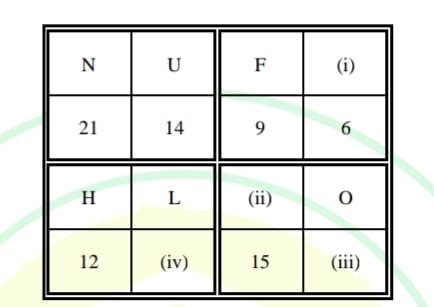
\includegraphics[width=0.7\columnwidth]{figs/2q-4.jpg}
        \caption{}
        \label{fig:q4}
    \end{figure}

    \hfill{\brak{\text{GATE CE 2025}}}
    \begin{enumerate}
        \item Q, M, $12$, and $8$
        \item K, L, $10$ and $14$
        \item I, J, $10$, and $8$
        \item L, K, $12$ and $8$
    \end{enumerate}

    \item A bag contains Violet \brak{V}, Yellow \brak{Y}, Red \brak{R}, and Green \brak{G} balls. On counting them, the following results are obtained:
    \begin{enumerate}
        \item[(i)] The sum of Yellow balls and twice the number of Violet balls is $50$.
        \item[(ii)] The sum of Violet and Green balls is $50$.
        \item[(iii)] The sum of Yellow and Red balls is $50$.
        \item[(iv)] The sum of Violet and twice the number of Red balls is $50$.
    \end{enumerate}
    Which one of the following Pie charts correctly represents the balls in the bag?

    \hfill{\brak{\text{GATE CE 2025}}}
   \begin{enumerate}
       \item \begin{figure}[H]
        \centering
        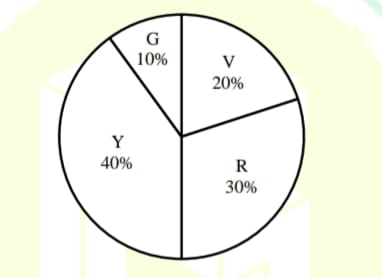
\includegraphics[width=0.7\columnwidth]{figs/2q-5a.jpg}
        \caption{}
        \label{fig:q4}
    \end{figure}
     \item \begin{figure}[H]
        \centering
        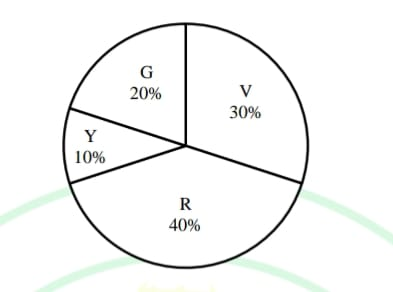
\includegraphics[width=0.7\columnwidth]{figs/2q-5b.jpg}
        \caption{}
        \label{fig:q4}
    \end{figure}
     \item \begin{figure}[H]
        \centering
        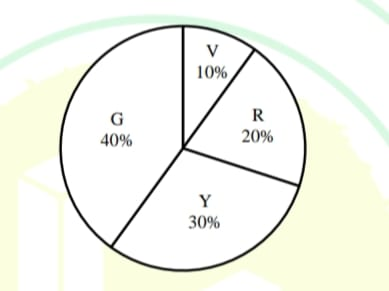
\includegraphics[width=0.7\columnwidth]{figs/2q-5c.jpg}
        \caption{}
        \label{fig:q4}
    \end{figure}
     \item \begin{figure}[H]
        \centering
        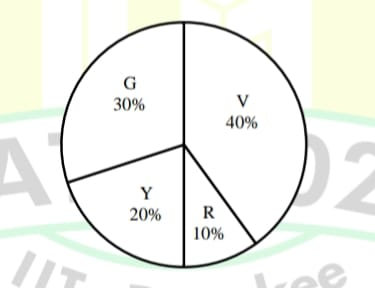
\includegraphics[width=0.7\columnwidth]{figs/2q-5d.jpg}
        \caption{}
        \label{fig:q4}
    \end{figure}
   \end{enumerate}

    \item "His life was divided between the books, his friends, and long walks. A solitary man, he worked at all hours without much method, and probably courted his fatal illness in this way. To his own name there is not much to show; but such was his liberality that he was continually helping others, and fruits of his erudition are widely scattered, and have gone to increase many a comparative stranger's reputation."
    
    \brak{\text{From E.V. Lucas's "A Funeral"}}
    
    Based only on the information provided in the above passage, which one of the following statements is true?

    \hfill{\brak{\text{GATE CE 2025}}}
    \begin{enumerate}
        \item The solitary man described in the passage is dead.
        \item Strangers helped create a grand reputation for the solitary man described in the passage.
        \item The solitary man described in the passage found joy in scattering fruits.
        \item The solitary man worked in a court where he fell ill.
    \end{enumerate}

    \item For the clock shown in the figure \figref{fig:q7}, if
    $O^* = O \, Q \, S \, Z \, P \, R \, T$, and
    $X^* = X \, Z \, P \, W \, Y \, O \, Q$,
    then which one among the given options is most appropriate for $P^*$?
    \begin{figure}[H]
        \centering
        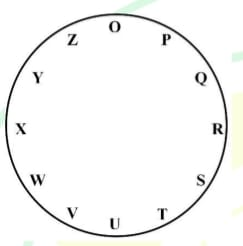
\includegraphics[width=0.7\columnwidth]{figs/2q-7.jpg}
        \caption{}
        \label{fig:q7}
    \end{figure}

    \hfill{\brak{\text{GATE CE 2025}}}
    \begin{enumerate}
        \begin{multicols}{2}
            \item P U W R T V X
            \item P R T O Q S U
            \item P T V Q S U W
            \item P S U P R T V
        \end{multicols}
    \end{enumerate}

    \item Consider a five-digit number $PQRST$ that has distinct digits $P, Q, R, S$, and $T$, and satisfies the following conditions:
    \begin{align*}
        P &< Q \\
        S &> P > T \\
        R &< T
    \end{align*}
    If integers $1$ through $5$ are used to construct such a number, the value of $P$ is:
    
    \hfill{\brak{\text{GATE CE 2025}}}
    \begin{enumerate}
        \begin{multicols}{4}
            \item $1$
            \item $2$
            \item $3$
            \item $4$
        \end{multicols}
    \end{enumerate}

    \item A business person buys potatoes of two different varieties P and Q, mixes them in a certain ratio and sells them at Rs $192$ per kg.
    The cost of the variety P is Rs $800$ for $5$ kg.
    The cost of the variety Q is Rs $800$ for $4$ kg.
    If the person gets $8$\% profit, what is the P:Q ratio \brak{by weight}?
    
    \hfill{\brak{\text{GATE CE 2025}}}
    \begin{enumerate}
        \begin{multicols}{4}
            \item $5:4$
            \item $3:4$
            \item $3:2$
            \item $1:1$
        \end{multicols}
    \end{enumerate}

    \item Three villages P, Q, and R are located in such a way that the distance PQ $= 13$ km, QR $= 14$ km, and RP $= 15$ km, as shown in the figure \figref{fig:q10}. A straight road joins Q and R. It is proposed to connect P to this road QR by constructing another road. What is the minimum possible length \brak{in km} of this connecting road?
    
    Note: The figure shown is representative.
    \begin{figure}[H]
        \centering
        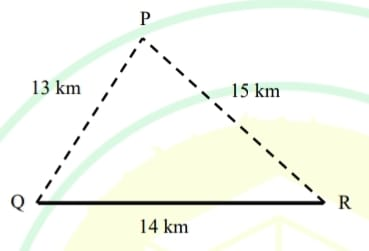
\includegraphics[width=0.7\columnwidth]{figs/2q-10.jpg}
        \caption{}
        \label{fig:q10}
    \end{figure}

    \hfill{\brak{\text{GATE CE 2025}}}
    \begin{enumerate}
        \begin{multicols}{4}
            \item $10.5$
            \item $11.0$
            \item $12.0$
            \item $12.5$
        \end{multicols}
    \end{enumerate}

    \item For the matrix $[A]$ given below, the transpose is \underline{\hspace{2cm}}.
    \[ [A] = \myvec{2 & 3 & 4 \\ 1 & 4 & 5 \\ 4 & 3 & 2} \]

    \hfill{\brak{\text{GATE CE 2025}}}
    \begin{enumerate}
        \item $\myvec{2 & 1 & 4 \\ 3 & 4 & 3 \\ 4 & 5 & 2}$
        \item $\myvec{4 & 3 & 2 \\ 5 & 4 & 1 \\ 2 & 3 & 4}$
        \item $\myvec{4 & 2 & 3 \\ 5 & 1 & 4 \\ 2 & 4 & 3}$
        \item $\myvec{2 & 3 & 4 \\ 1 & 4 & 5 \\ 4 & 3 & 2}$
    \end{enumerate}

    \item Integration of $\ln\brak{x}$ with x i.e.,
    \begin{align} \int \ln\brak{x} dx = \underline{\hspace{2cm}} \end{align}

    \hfill{\brak{\text{GATE CE 2025}}}
    \begin{enumerate}
        \begin{multicols}{2}
            \item $x \cdot \ln\brak{x} - x + \text{Constant}$
            \item $x - \ln\brak{x} + \text{Constant}$
            \item $x \cdot \ln\brak{x} + x + \text{Constant}$
            \item $\ln\brak{x} - x + \text{Constant}$
        \end{multicols}
    \end{enumerate}

    \item Consider the following statements \brak{P} and \brak{Q}:
    \brak{P}: Fly ash and ground granulated blast furnace slag can be used as mineral admixtures in concrete.
    \brak{Q}: As per IS 456:2000, the minimum moist curing period becomes higher when a mineral admixture is added to concrete.
    Identify the CORRECT option from choices given below.

    \hfill{\brak{\text{GATE CE 2025}}}
    \begin{enumerate}
        \item Both \brak{P} and \brak{Q} are TRUE.
        \item \brak{P} is TRUE and \brak{Q} is FALSE.
        \item \brak{P} is FALSE and \brak{Q} is TRUE.
        \item Both \brak{P} and \brak{Q} are FALSE.
    \end{enumerate}

    \item Consider the pin-jointed truss shown in the figure \figref{fig:q14}. Influence line is drawn for the axial force in the member G-I, when a unit load travels on the bottom chord of the truss. Identify the CORRECT influence line from the following options:
    
    Note: Positive value corresponds to tension and negative value corresponds to compression in the member.
    \begin{figure}[H]
        \centering
        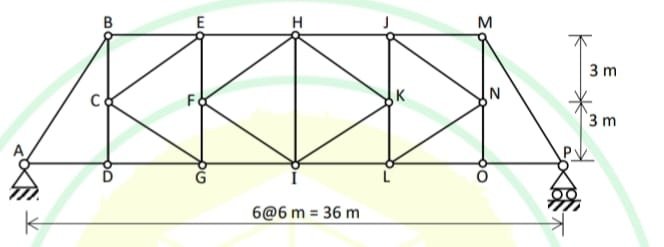
\includegraphics[width=0.7\columnwidth]{figs/2q-14.jpg}
        \caption{}
        \label{fig:q14}
    \end{figure}

    \hfill{\brak{\text{GATE CE 2025}}}
    \begin{enumerate}
        \item \begin{figure}[H]
        \centering
        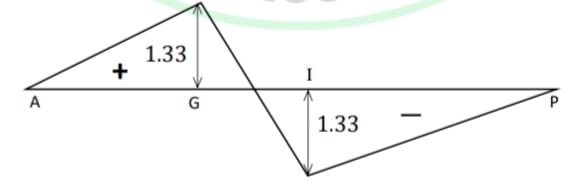
\includegraphics[width=0.7\columnwidth]{figs/2q-14a.jpg}
        \caption{}
        \label{fig:q14}
    \end{figure}
    \item \begin{figure}[H]
        \centering
        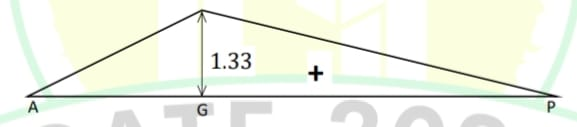
\includegraphics[width=0.7\columnwidth]{figs/2q-14b.jpg}
        \caption{}
        \label{fig:q14}
    \end{figure}
    \item \begin{figure}[H]
        \centering
        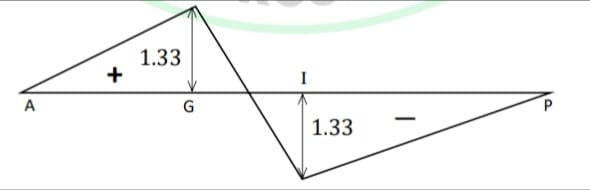
\includegraphics[width=0.7\columnwidth]{figs/2q-14c.jpg}
        \caption{}
        \label{fig:q14}
    \end{figure}
    \item \begin{figure}[H]
        \centering
        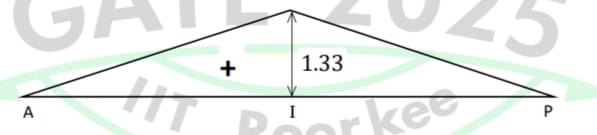
\includegraphics[width=0.7\columnwidth]{figs/2q-14d.jpg}
        \caption{}
        \label{fig:q14}
    \end{figure}
    \end{enumerate}

    \item The most suitable test for measuring the permeability of clayey soils in the laboratory is \underline{\hspace{2cm}}.

    \hfill{\brak{\text{GATE CE 2025}}}
    \begin{enumerate}
        \begin{multicols}{2}
            \item Constant head test
            \item Pumping out test
            \item Hydrometer test
            \item Falling head test
        \end{multicols}
    \end{enumerate}

    \item A hydraulic jump occurs in an open channel when the slope of the channel changes from \underline{\hspace{2cm}}.

    \hfill{\brak{\text{GATE CE 2025}}}
    \begin{enumerate}
        \begin{multicols}{2}
            \item MILD slope to STEEP slope
            \item STEEP slope to MILD slope
            \item MILD slope to ZERO slope
            \item STEEP slope to a STEEPER slope
        \end{multicols}
    \end{enumerate}

    \item The bacteria mainly responsible for crown corrosion in a sewer is \underline{\hspace{2cm}}.

    \hfill{\brak{\text{GATE CE 2025}}}
    \begin{enumerate}
        \begin{multicols}{2}
            \item Methanogenic bacteria
            \item Denitrifying bacteria
            \item Sulphur reducing bacteria
            \item \textit{Pseudomonas} bacteria
        \end{multicols}
    \end{enumerate}

    \item The recommended minimum traffic growth rate and design period considered for structural design of flexible pavements for national highways in India as per IRC 37:2018 is \underline{\hspace{1cm}} percentage and \underline{\hspace{1cm}} years, respectively.

    \hfill{\brak{\text{GATE CE 2025}}}
    \begin{enumerate}
        \begin{multicols}{2}
            \item $5, 20$
            \item $5, 30$
            \item $7, 20$
            \item $7, 30$
        \end{multicols}
    \end{enumerate}

    \item After applying the correction for elevation and temperature, the runway length is $700$ m. The corrected runway length \brak{in m} for an effective gradient of $1$\% is \underline{\hspace{2cm}} \\ \brak{\text{round off to the nearest integer}}.

    \hfill{\brak{\text{GATE CE 2025}}}
    \begin{enumerate}
        \begin{multicols}{4}
            \item $840$
            \item $700$
            \item $720$
            \item $740$
        \end{multicols}
    \end{enumerate}

    \item The point where the road alignment changes from a tangent to a curve is known as \underline{\hspace{2cm}}.

    \hfill{\brak{\text{GATE CE 2025}}}
    \begin{enumerate}
        \begin{multicols}{2}
            \item Point of deflection
            \item Point of intersection
            \item Point of curve
            \item Point of tangency
        \end{multicols}
    \end{enumerate}

    \item Consider a velocity vector, $\vec{V}$ in $\brak{x, y, z}$ coordinates given below. Pick one or more CORRECT statements\brak{s} from the choices given below.
    \begin{align} \vec{V} = u\vec{x} + v\vec{y} \end{align}

    \hfill{\brak{\text{GATE CE 2025}}}
    \begin{enumerate}
        \item z-component of Curl of velocity; $\nabla \times \vec{V} = \brak{\frac{\partial v}{\partial x} - \frac{\partial u}{\partial y}}\vec{z}$
        \item z-component of Curl of velocity; $\nabla \times \vec{V} = \brak{\frac{\partial u}{\partial x} - \frac{\partial v}{\partial y}}\vec{z}$
        \item Divergence of velocity; $\nabla \cdot \vec{V} = \brak{\frac{\partial u}{\partial x} + \frac{\partial v}{\partial y}}$
        \item Divergence of velocity; $\nabla \cdot \vec{V} = \brak{\frac{\partial u}{\partial y} + \frac{\partial v}{\partial x}}$
    \end{enumerate}

    \item Given that A and B are not null sets, which of the following statements regarding probability is/are CORRECT?

    \hfill{\brak{\text{GATE CE 2025}}}
    \begin{enumerate}
        \item $P\brak{A \cap B} = P\brak{A} P\brak{B}$, if A and B are mutually exclusive.
        \item Conditional probability, $P\brak{A|B} = 1$ if $B \subseteq A$.
        \item $P\brak{A \cup B} = P\brak{A} + P\brak{B}$, if A and B are mutually exclusive.
        \item $P\brak{A \cap B} = 0$, if A and B are independent.
    \end{enumerate}

    \item In the context of construction materials, which of the following statements is/are CORRECT?

    \hfill{\brak{\text{GATE CE 2025}}}
    \begin{enumerate}
        \item If the characteristic strength is defined as that value below which not more than $50$\% results are expected to fall, the target mean strength in mix design will be taken same as the characteristic strength irrespective of the degree of quality control expected at the site.
        \item Ten percent fines value is a non-dimensional quantity.
        \item The stress-strain curve of concrete for $1$-day duration of loading is associated with a smaller secant modulus of elasticity compared to the stress-strain curve of the same concrete for $10$-minutes duration of loading.
        \item The increase of carbon in steel usually leads to an increase in its $0.2$\% proof stress.
    \end{enumerate}

    \item Which of the following statements is/are INCORRECT?

    \hfill{\brak{\text{GATE CE 2025}}}
    \begin{enumerate}
        \item As the depth of the ground water table from the ground surface increases, the effective stress in the soil decreases.
        \item Bulking of the moist sand is due to the capillary action in the sand.
        \item The effective stress in a liquified soil is almost zero.
        \item The earth pressure at any point in the soil, under all conditions, is always smaller than the vertical effective stress at that point.
    \end{enumerate}

    \item Pick one or more CORRECT statement\brak{s} from the choices given below, in the context of upstream and downstream cut-offs provided below the concrete apron of weirs / barrages constructed across alluvial rivers.

    \hfill{\brak{\text{GATE CE 2025}}}
    \begin{enumerate}
        \item Cut-offs are provided to increase the rate of flow over the weir / barrage.
        \item Cut-offs are provided to increase the seepage length and prevent failure due to piping.
        \item The bottom level of cut-offs mainly depends on the scour depth.
        \item Cut-offs are provided to ensure occurrence of hydraulic jump within the stilling basin.
    \end{enumerate}

    \item In the context of the effect of drainage density on the run-off generation and the hydrograph at the catchment outlet, all other factors remaining the same, pick one or more CORRECT statement\brak{s} from the choices given below.

    \hfill{\brak{\text{GATE CE 2025}}}
    \begin{enumerate}
        \item Lower drainage density results in higher peak in flood hydrograph compared to that when the drainage density is higher.
        \item Lower drainage density results in lower peak in flood hydrograph compared to that when the drainage density is higher.
        \item Lower drainage density results in a flood hydrograph with a longer time base compared to that when the drainage density is higher.
        \item Lower drainage density results in a flood hydrograph with a shorter time base compared to that when the drainage density is higher.
    \end{enumerate}

    \item Identify the treatment technology/technologies NOT recommended for highly biodegradable organic solid wastes.

    \hfill{\brak{\text{GATE CE 2025}}}
    \begin{enumerate}
        \begin{multicols}{2}
            \item Biohydrogenation
            \item Anaerobic digestion
            \item Composting
            \item Open dumping
        \end{multicols}
    \end{enumerate}

    \item Which of the following statements is/are INCORRECT?

    \hfill{\brak{\text{GATE CE 2025}}}
    \begin{enumerate}
        \item Bitumen having lower softening point is preferred in warm climate regions.
        \item The viscosity of bitumen influences the mixing and compaction of bituminous mix.
        \item The air voids in the range of $3$\% to $5$\% are required to arrive at the optimum bitumen content.
        \item The purity of bitumen can be determined using Solubility Test.
    \end{enumerate}

    \item The "order" of the following ordinary differential equation is \underline{\hspace{2cm}}.
    \begin{align} 
    \frac{d^3y}{dx^3} + \brak{\frac{d^2y}{dx^2}}^6 + \brak{\frac{dy}{dx}}^4 + y = 0 
    \end{align}
    
    \hfill{\brak{\text{GATE CE 2025}}}

    \item The design shear strength of a reinforced concrete rectangular beam with a width of $250$ mm and an effective depth of $500$ mm, is $0.3$ MPa. The torsional moment capacity of the section \brak{in kN.m} under pure torsion, as per IS 456:2000, is \underline{\hspace{2cm}} \\ \brak{\text{round off to one decimal place}}.
    
    \hfill{\brak{\text{GATE CE 2025}}}

    \item From a flow-net diagram drawn under a concrete dam, following information are obtained: \brak{i} The head difference between upstream and downstream side of the dam is $9$ m. \brak{ii} The total number of equipotential drops between upstream and downstream side of the dam is $10$. \brak{iii} The length of the field nearest to the toe of the dam in the downstream side is $1$ m.
    
    If the soil below the dam is having a saturated unit weight of $21$ kN/m$^3$ and unit weight of water is $9.81$ kN/m$^3$, then the factor of safety against the quick condition will be \underline{\hspace{2cm}} \\ \brak{\text{round off to two decimal place}}.
    
    \hfill{\brak{\text{GATE CE 2025}}}

    \item A $6$ m thick clay stratum has drainage at both its top and bottom surface due to the presence of sand strata. The time to complete $50$\% consolidation is $2$ years. The coefficient of volume change \brak{m_v} is $1.51 \times 10^{-3}$ m$^2$/kN and unit weight of water is $9.81$ kN/m$^3$.
    
    The coefficient of permeability \brak{\text{in m/year}} is \underline{\hspace{2cm}} \\
    \brak{\text{round off to three decimal places}}.
    
    \hfill{\brak{\text{GATE CE 2025}}}

    \item Consider steady flow of water in the series pipe system shown below \figref{fig:q33}, with specified discharge. The diameters of Pipes A and B are $2$ m and $1$ m, respectively. The lengths of pipes A and B are $100$ m and $200$ m, respectively. Assume the Darcy-Weisbach friction coefficient, $f$ as $0.01$ for both the pipes.
    
    The ratio of head loss in Pipe-B to the head loss in Pipe-A is \underline{\hspace{2cm}} \\ \brak{\text{round off to the nearest integer}}.
    \begin{figure}[H]
        \centering
        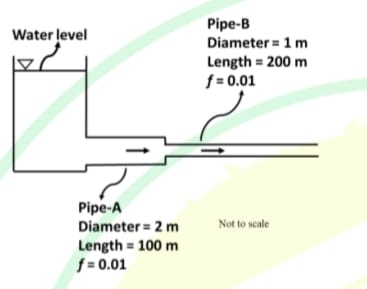
\includegraphics[width=0.7\columnwidth]{figs/2q-33.jpg}
        \caption{}
        \label{fig:q33}
    \end{figure}
    
    \hfill{\brak{\text{GATE CE 2025}}}

    \item Free residual chlorine concentration in water was measured to be $2$ mg/l \brak{\text{as $Cl_2$}}. The pH of water is $8.5$. By using the chemical equation given below, the HOCl concentration \brak{\text{in \micro moles/l}} in water is \underline{\hspace{2cm}}\\ \brak{\text{round off to one decimal place}}.
    \begin{align}
    HOCl \rightleftharpoons H^+ + OCl^- \quad pK = 7.50 
    \end{align}
    Atomic weight: Cl\brak{35.5}
   
    \hfill{\brak{\text{GATE CE 2025}}}

    \item A surveyor measured the distance between two points on the plan drawn to a scale of $1$ cm $= 40$ m and the result was $468$ m. Later, it was discovered that the scale used was $1$ cm $= 20$ m.
    
    The true distance between the points \brak{in m} is \underline{\hspace{2cm}} \\ \brak{\text{round off to the nearest integer}}.
    
    \hfill{\brak{\text{GATE CE 2025}}}
    
    \item Pick the CORRECT solution for the following differential equation
    \begin{align}
    \frac{dy}{dx} = e^{x-y} 
    \end{align}

    \hfill{\brak{\text{GATE CE 2025}}}
    \begin{enumerate}
        \begin{multicols}{2}
            \item $y = \ln\brak{e^x + \text{Constant}}$
            \item $\ln\brak{y} = x + \text{Constant}$
            \item $\ln\brak{y} = \ln\brak{e^x} + \text{Constant}$
            \item $y = x + \text{Constant}$
        \end{multicols}
    \end{enumerate}

    \item A circular tube of thickness $10$ mm and diameter $250$ mm is welded to a flat plate using $5$ mm fillet weld along the circumference. Assume Fe410 steel and shop welding.
    As per IS 800:2007, the torque that can be resisted by the weld \brak{\text{in kN.m}} is \underline{\hspace{2cm}} \\ \brak{\text{round off to one decimal place}}.

    \hfill{\brak{\text{GATE CE 2025}}}
    \begin{enumerate}
        \begin{multicols}{2}
            \item $65.1$
            \item $78.1$
            \item $156.2$
            \item $130.2$
        \end{multicols}
    \end{enumerate}

    \item The figure \figref{fig:q38} shows a propped cantilever with uniform flexural rigidity $EI$ \brak{\text{in N.$m^2$}} and subjected to a moment $M$ \brak{\text{in N.m}}. Consider forces and displacements in the upward direction as positive.
    Find the upward reaction at the propped support B \brak{\text{in N}} when this support settles by \brak{-\Delta}, given in metres.
    \begin{figure}[H]
        \centering
        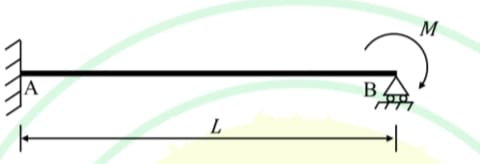
\includegraphics[width=0.7\columnwidth]{figs/2q-38.jpg}
        \caption{}
        \label{fig:q38}
    \end{figure}

    \hfill{\brak{\text{GATE CE 2025}}}
    \begin{enumerate}
        \item $\frac{3M}{2L} - \frac{6EI\Delta}{L^3}$
        \item $\frac{8M}{3L} - \frac{2EI\Delta}{L^3}$
        \item $\frac{3M}{2L} - \frac{3EI\Delta}{L^3}$
        \item $\frac{M}{L} - \frac{8EI\Delta}{L^3}$
    \end{enumerate}

    \item Let the state of stress at a point in a body be the difference of two plane states of stress shown in the figure \figref{fig:q39}. Consider all the possible planes perpendicular to the x-y plane and passing through that point. The magnitude of the maximum compressive stress on any such plane is $k\sigma_0$, where $k$ is equal to \underline{\hspace{2cm}} \\ \brak{\text{round off to one decimal place}}.
    \begin{figure}[H]
        \centering
        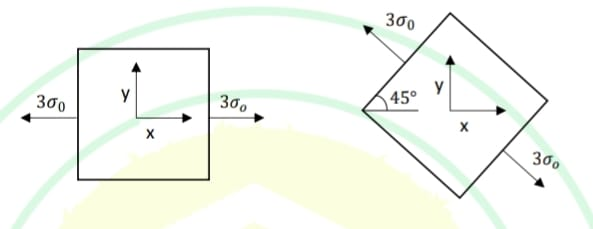
\includegraphics[width=0.7\columnwidth]{figs/2q-39.jpg}
        \caption{}
        \label{fig:q39}
    \end{figure}
    
    \hfill{\brak{\text{GATE CE 2025}}}
    \begin{enumerate}
        \begin{multicols}{4}
            \item $3.0$
            \item $2.1$
            \item $1.7$
            \item $1.5$
        \end{multicols}
    \end{enumerate}

    \item Consider a reinforced concrete beam section of $350$ mm width and $600$ mm depth. The beam is reinforced with the tension steel of $800$ mm$^2$ area at an effective cover of $40$ mm. Consider M20 concrete and Fe415 steel. Let the stress block considered for concrete in IS 456:2000 be replaced by an equivalent rectangular stress block, with no change in \brak{a} the area of the stress block, \brak{b} the design strength of concrete \brak{\text{at the strain of $0.0035$}}, and \brak{c} the location of neutral axis at flexural collapse. The ultimate moment of resistance of the beam \brak{\text{in kN.m}} is \underline{\hspace{2cm}} \\ \brak{\text{round off to the nearest integer}}.

    \hfill{\brak{\text{GATE CE 2025}}}
    \begin{enumerate}
        \begin{multicols}{4}
            \item $170$
            \item $148$
            \item $125$
            \item $102$
        \end{multicols}
    \end{enumerate}

    \item For a partially saturated soil deposit at a construction site, water content \brak{w} is $15$\%, degree of saturation \brak{S} is $67$\%, void ratio \brak{e} is $0.6$ and specific gravity of solids in the soil \brak{G_s} is $2.67$. Consider unit weight of water as $9.81$ kN/m$^3$.
    
    To fully saturate $5$ m$^3$ of this soil, the required weight of water \brak{in kN} will be \underline{\hspace{2cm}} \\ \brak{\text{round off to the nearest integer}}.
    
    \hfill{\brak{\text{GATE CE 2025}}}
    \begin{enumerate}
        \begin{multicols}{4}
            \item $5$
            \item $6$
            \item $7$
            \item $8$
        \end{multicols}
    \end{enumerate}

    \item Consider flow in a long and very wide rectangular open channel. Width of the channel can be considered as infinity compared to the depth of flow. Uniform flow depth is $1.0$ m. The bed slope of the channel is $0.0001$. The Manning roughness coefficient value is $0.02$. Acceleration due to gravity, g can be taken as $9.81$ m/s$^2$.
    
    The critical depth \brak{\text{in m}} corresponding to the flow rate resulting from the above conditions is \underline{\hspace{2cm}} \\ \brak{\text{round off to one decimal place}}.
    
    \hfill{\brak{\text{GATE CE 2025}}}
    \begin{enumerate}
        \begin{multicols}{4}
            \item $0.4$
            \item $0.3$
            \item $0.6$
            \item $0.1$
        \end{multicols}
    \end{enumerate}

    \item Match the following in Column I with Column II.
    \begin{center}
    \begin{tabular}{|l|l|}
        \hline
        \textbf{Column I} & \textbf{Column II} \\
        \hline
        (1) Vehicle Damage Factor & A. Stability of subgrade soil \\
        (2) Passenger Car Unit & B. Capacity of a roadway \\
        (3) Perception Reaction Time & C. Design rigid pavement \\
        (4) California Bearing Ratio & D. Design flexible pavement \\
        & E. Stopping sight distance \\
        \hline
    \end{tabular}
    \end{center}

    \hfill{\brak{\text{GATE CE 2025}}}
    \begin{enumerate}
        \item (1)-(D); (2)-(B); (3)-(E); (4)-(A)
        \item (1)-(C); (2)-(B); (3)-(D); (4)-(A)
        \item (1)-(D); (2)-(E); (3)-(B); (4)-(A)
        \item (1)-(D); (2)-(B); (3)-(A); (4)-(E)
    \end{enumerate}

    \item Consider the function given below and pick one or more CORRECT statement\brak{s} from the following choices.
    \begin{align} 
    f\brak{x} = x^3 - \frac{15}{2}x^2 + 18x + 20 
    \end{align}

    \hfill{\brak{\text{GATE CE 2025}}}
    \begin{enumerate}
        \item $f\brak{x}$ has a local minimum at $x=3$.
        \item $f\brak{x}$ has a local maximum at $x=3$.
        \item $f\brak{x}$ has a local minimum at $x=2$.
        \item $f\brak{x}$ has a local maximum at $x=2$.
    \end{enumerate}

    \item Pick the CORRECT eigen value\brak{s} of the matrix $[A]$ from the following choices.
    \begin{align}
    [A] = \myvec{6 & 8 \\ 4 & 2} 
    \end{align}

    \hfill{\brak{\text{GATE CE 2025}}}
    \begin{enumerate}
        \begin{multicols}{4}
            \item $10$
            \item $4$
            \item $-2$
            \item $-10$
        \end{multicols}
    \end{enumerate}

    \item In the pin-jointed truss shown in the figure \figref{fig:q46}, the members that carry zero force are identified. Which of the following options is/are zero-force members?
    \begin{figure}[H]
        \centering
        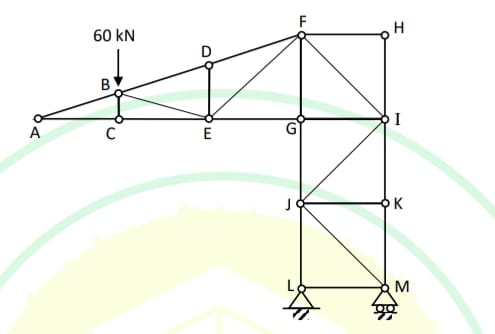
\includegraphics[width=0.7\columnwidth]{figs/2q-46.jpg}
        \caption{}
        \label{fig:q46}
    \end{figure}

    \hfill{\brak{\text{GATE CE 2025}}}
    \begin{enumerate}
        \begin{multicols}{4}
            \item BC
            \item EG
            \item FI
            \item JK
        \end{multicols}
    \end{enumerate}

    \item In the context of shear strength of soil, which of the following statements is/are CORRECT?

    \hfill{\brak{\text{GATE CE 2025}}}
    \begin{enumerate}
        \item The unconfined compression test is a special case of the unconsolidated-undrained \brak{UU} triaxial tests.
        \item The shear strength parameters obtained from the consolidated-drained \brak{CD} triaxial tests should be used to analyse rapid construction in clay.
        \item Vane shear test is commonly used for determining in situ undrained strength of saturated clay soils.
        \item In an unconsolidated-undrained \brak{UU} triaxial tests, the angle of internal friction \brak{\phi} is equal to zero.
    \end{enumerate}

    \item The drag force, $F_D$ on a sphere due to a fluid flowing past the sphere is a function of viscosity, $\mu$, the mass density, $\rho$, the velocity of flow, $V$, and the diameter of the sphere, $D$.
    
    Pick the relevant \brak{\text{one or more}} non-dimensional parameter\brak{s} pertaining to the above process from the following list.
    
    \hfill{\brak{\text{GATE CE 2025}}}
    \begin{enumerate}
        \item $\frac{F_D}{\rho V^2 D^2}$
        \item $\frac{\rho F_D}{V^2 D^2}$
        \item $\frac{\rho V D}{\mu}$
        \item $\frac{\mu \rho}{V D}$
    \end{enumerate}

    \item A compound has a general formula C$_a$H$_b$O$_c$N$_d$ and molecular weight $187$. A $935$ mg/l solution of the compound is prepared in distilled deionized water. The Total Organic Carbon \brak{TOC} is measured as $360$ mg/l \brak{\text{as C}}. The Chemical Oxygen Demand \brak{COD} and the Total Kjeldahl Nitrogen \brak{TKN} are determined as $600$ mg/l \brak{\text{as O$_2$}} and $140$ mg/l \brak{as N}, respectively \brak{\text{as per the chemical equation given below}}. Which of the following options is/are CORRECT?
    \[ \text{C}_a\text{H}_b\text{O}_c\text{N}_d + \frac{\brak{4a+b-2c-3d}}{4}\text{O}_2 \rightarrow a\text{CO}_2 + \frac{b-3d}{2}\text{H}_2\text{O} + d\text{NH}_3 \]
    Atomic weight: C\brak{12}, H\brak{1}, O\brak{16}, N\brak{14}
    
    \hfill{\brak{\text{GATE CE 2025}}}
    \begin{enumerate}
        \begin{multicols}{4}
            \item $a=6$
            \item $b=7$
            \item $c=5$
            \item $d=3$
        \end{multicols}
    \end{enumerate}

    \item The free flow speed of a highway is $100$ km/h and its capacity is $4000$ vehicle/h. Assume speed density relation is linear.
    For a traffic volume of $2000$ vehicle/h, choose all the possible speeds \brak{\text{in km/h}} from the options given below \\ \brak{\text{round off to two decimal place}}.
    
    \hfill{\brak{\text{GATE CE 2025}}}
    \begin{enumerate}
        \begin{multicols}{2}
            \item $85.36$
            \item $65.20$
            \item $14.64$
            \item $7.22$
        \end{multicols}
    \end{enumerate}

    \item Consider a discrete random variable $X$ whose probabilities are given below. The standard deviation of the random variable is \underline{\hspace{2cm}} \\ \brak{\text{round off to one decimal place}}.
    \begin{center}
    \begin{tabular}{|c|c|c|c|c|}
        \hline
        $x_i$ & $1$ & $2$ & $4$ & $8$ \\
        \hline
        $P\brak{X=x_i}$ & $0.3$ & $0.1$ & $0.3$ & $0.3$ \\
        \hline
    \end{tabular}
    \end{center}
    
    \hfill{\brak{\text{GATE CE 2025}}}

    \item A steel beam supported by three parallel pin-jointed steel rods is shown in the figure \figref{fig:q52}. The moment of inertia of the beam is $8 \times 10^7$ mm$^4$. Take modulus of elasticity of steel as $210$ GPa. The beam is subjected to uniformly distributed load of $6.25$ kN/m, including its self-weight.
    
    The axial force \brak{in kN} in the centre rod CD is \underline{\hspace{2cm}} \\ \brak{\text{round off to one decimal place}}.
    \begin{figure}[H]
        \centering
        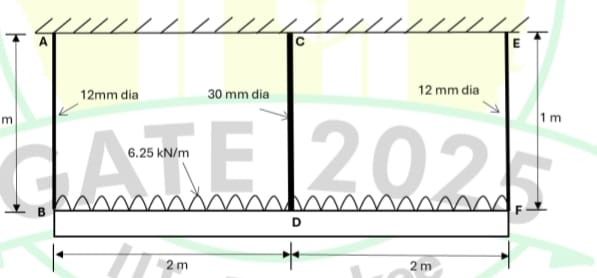
\includegraphics[width=0.7\columnwidth]{figs/2q-52.jpg}
        \caption{}
        \label{fig:q52}
    \end{figure}
    
    \hfill{\brak{\text{GATE CE 2025}}}

    \item The figure shows a network diagram for a construction project. The activities A, B, C, D, E, and F are represented by arrows and their durations are in the figure \figref{fig:q53}.
    
    The total float available for the activity E in day\brak{s} is equal to \underline{\hspace{2cm}} \\ \brak{\text{round off to the nearest integer}}.
    \begin{figure}[H]
        \centering
        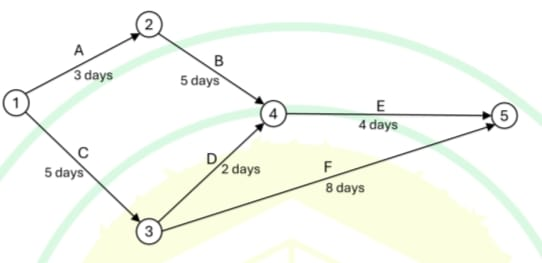
\includegraphics[width=0.7\columnwidth]{figs/2q-53.jpg}
        \caption{}
        \label{fig:q53}
    \end{figure}
    
    \hfill{\brak{\text{GATE CE 2025}}}

    \item A reinforced concrete beam has a support section with width of $300$ mm and effective depth of $500$ mm. The support section is reinforced with $3$ bars of $20$ mm diameter at the tension side. Two-legged vertical stirrups of $10$ mm diameter and Fe415 steel at a spacing of $100$ mm are provided as shear reinforcement. Assume that there is no possibility of diagonal compression failure at the section.
    
    As per IS 456:2000, the maximum shear resisted by the vertical stirrups , as per limit state design, is \underline{\hspace{2cm}} \\ \brak{\text{round off to one decimal place}}.
    
    \hfill{\brak{\text{GATE CE 2025}}}

    \item The bank of a canal has the profile shown in the figure \figref{fig:q55}. The material is a homogeneous clay with a bulk unit weight of $20$ kN/m$^3$, undrained cohesion of $30$ kPa and it is fully saturated \brak{\phi_u = 0}. For the trial slip circle shown, the area ABCDEA is $150$ m$^2$ and the centroid is at P. A tension crack \brak{DE} of $2.5$ m deep was also observed. Assume unit weight of water is $9.81$ kN/m$^3$ and consider $1$ m run of the bank for the analysis.
    
    Considering the canal is empty and tension crack is completely filled with water, the factor of safety against slope failure of the bank is \underline{\hspace{2cm}} \\ \brak{\text{round off to two decimal place}}.
    \begin{figure}[H]
        \centering
        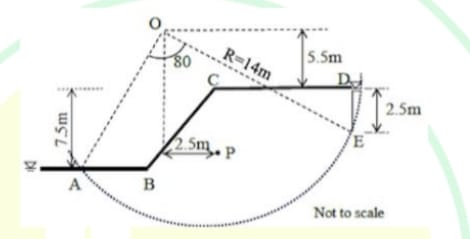
\includegraphics[width=0.7\columnwidth]{figs/2q-55.jpg}
        \caption{}
        \label{fig:q55}
    \end{figure}
    
    \hfill{\brak{\text{GATE CE 2025}}}
    
    \item A designer used plate load test to obtain the value of the bearing capacity factor $N_\gamma$. A circular plate of $1$ m diameter was placed on the surface of a dry sand layer extending very deep beneath the ground. The unit weight of the sand is $16.66$ kN/m$^3$. The plate is loaded to failure at a pressure of $1500$ kPa.
    
    Considering Terzaghi's bearing capacity theory, the bearing capacity factor $N_\gamma$ is \underline{\hspace{2cm}} \\ \brak{\text{round off to the nearest integer}}.
    
    \hfill{\brak{\text{GATE CE 2025}}}
    
    \item A $4 \times 4$ group pile, with each pile $20$ m long and $500$ mm in diameter, is installed in a square pattern in a clayey soil, as shown in the figure \figref{fig:q57}. The average unconfined compressive strength of the soil is $100$ kN/m$^2$, and the adhesion factor is $0.8$. Neglect the bearing at the tip of the piles. For a group efficiency factor of $1.0$, the centre to centre spacing \brak{s} of the piles \brak{\text{in m}} would be \underline{\hspace{2cm}} \\ \brak{\text{round off to two decimal place}}.
    \begin{figure}[H]
        \centering
        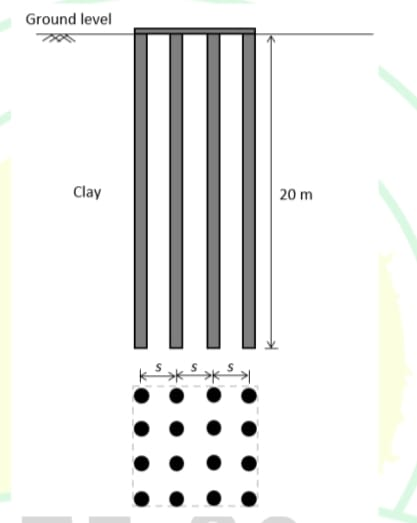
\includegraphics[width=0.7\columnwidth]{figs/2q-57.jpg}
        \caption{}
        \label{fig:q57}
    \end{figure}
    
    \hfill{\brak{\text{GATE CE 2025}}}
    
    \item A $60$ cm diameter well completely penetrates a confined aquifer of permeability $5 \times 10^{-4}$ m/s. The length of the strainer \\ \brak{\text{spanning the entire thickness of the aquifer}} is $10$ m. The drawdown at the well under steady state pumping is $1.0$ m. Assume that the radius of influence for this pumping is $300$ m.
    
    The discharge from the well \brak{\text{in litres per minute}} is \underline{\hspace{2cm}} \\ \brak{\text{round off to the nearest integer}}.
    
    \hfill{\brak{\text{GATE CE 2025}}}
    
    \item The peak of flood hydrograph due to a $3$-hour duration storm in a catchment is $180$ m$^3$/s. The total rainfall depth is $6.6$ cm. It can be assumed that the average infiltration loss is $0.2$ cm/h. There are no other losses. The base flow is constant at a value of $30$ m$^3$/s.
    
    The peak value of the $3$-hour unit hydrograph for this catchment \brak{\text{in m$^3$/s}} is \underline{\hspace{2cm}} \\ \brak{\text{round off to the nearest integer}}.
    
    \hfill{\brak{\text{GATE CE 2025}}}
    
    \item The shaft of a $6$ m wide gate in the figure \figref{fig:q60} will fail at a moment of $3924$ kN.m about the hinge P. The maximum value of water depth $h$ \brak{\text{in m}} that the gate can hold is \underline{\hspace{2cm}} \\ \brak{\text{round off to the nearest integer}}.
    
    Note:
    Density of water = $1000$ kg/m$^3$
    Acceleration due to gravity = $9.81$ m/s$^2$
    \begin{figure}[H]
        \centering
        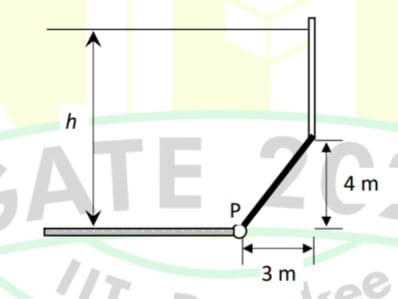
\includegraphics[width=0.7\columnwidth]{figs/2q-60.jpg}
        \caption{}
        \label{fig:q60}
    \end{figure}
    
    \hfill{\brak{\text{GATE CE 2025}}}
    
    \item The analyses results of a water sample are given below. The non-carbonate hardness of the water \brak{\text{in mg/L}} as CaCO$_3$ is \underline{\hspace{2cm}} \brak{in integer}.
    \begin{align*}
        \text{Ca}^{2+} &= 150 \text{ mg/L as CaCO}_3 \\
        \text{Mg}^{2+} &= 40 \text{ mg/L as CaCO}_3 \\
        \text{Fe}^{2+} &= 10 \text{ mg/L as CaCO}_3 \\
        \text{Na}^{+} &= 50 \text{ mg/L as CaCO}_3 \\
        \text{K}^{+} &= 10 \text{ mg/L as CaCO}_3 \\
        \text{CO}_3^{2-} &= 120 \text{ mg/L as CaCO}_3 \\
        \text{HCO}_3^{-} &= 30 \text{ mg/L as CaCO}_3 \\
        \text{Cl}^{-} &= 50 \text{ mg/L as CaCO}_3; \text{ Other anions were not analysed.}
    \end{align*}
    
    \hfill{\brak{\text{GATE CE 2025}}}
    
    \item A community generates $1$ million litres/day \brak{MLD} of wastewater. This wastewater is treated using activated sludge process \brak{ASP}. The working volume of the aeration tank of the ASP is $250$ m$^3$, and the biomass concentration in the tank is $3000$ mg/L. Analyses results showed that a biomass concentration of $10$ mg/L is present in the treated effluent from the secondary sedimentation tank of the ASP. Sludge wastage from the system is at a rate of $5000$ L/day with a biomass concentration of $10000$ mg/L. The system is in steady state condition.
    
    The biological sludge residence time \brak{BSRT} of the system \brak{\text{in days}} is \underline{\hspace{2cm}} \\ \brak{\text{round off to one decimal place}}.
    
    \hfill{\brak{\text{GATE CE 2025}}}
    
    \item A settling chamber is used for the removal of discrete particulate matter from air with following conditions. Horizontal velocity of air $= 0.2$ m/s; Temperature of air stream $= 77\degree$C; Specific gravity of particle to be removed $= 2.65$; Chamber length $= 12$ m; Chamber height $= 2$ m; Viscosity of air at $77\degree$C $= 2.1 \times 10^{-5}$ kg/m.s; Acceleration due to gravity \brak{g} $= 9.81$ m/s$^2$; Density of air at $77\degree$C $= 1.0$ kg/m$^3$; Assume the density of water as $1000$ kg/m$^3$ and Laminar condition exists in the chamber.
    
    The minimum size of particle that will be removed with $100$\% efficiency in the settling chamber \brak{\text{in \micro m}} is \underline{\hspace{2cm}} \\ \brak{\text{round off to one decimal place}}.
    
    \hfill{\brak{\text{GATE CE 2025}}}
    
    \item On a two-lane highway, a horizontal curve of radius $300$ m is provided. The design speed is $80$ km/h.
    
    If the longest wheelbase of vehicle expected on this highway is $7$ m, then the extra widening required \brak{\text{in m}} is \underline{\hspace{2cm}} \\ \brak{\text{round off to two decimal place}}.
    
    \hfill{\brak{\text{GATE CE 2025}}}
    
    \item If the Fore Bearing of the lines AB and BC are $60\degree$ and $122\degree$, respectively, then the interior angle $\angle$ABC \brak{\text{in degrees}} is \underline{\hspace{2cm}} \\ \brak{\text{round off to the nearest integer}}.
    
    \hfill{\brak{\text{GATE CE 2025}}}
    
\end{enumerate}

\end{document}
